
\section{Ejercicio 3}

\subsection{Desarrollo}
Para poder resolver el problema de TaskBatch lo que hacemos es generar cant$\_$bloqueos valores aleatorios no repetidos que no estén ubicados fuera de total$\_$cpu. 
Lo generado por esto podría no estar ordenado, así que le hacemos un sort al resultado. Por último ciclaremos total$\_$cpu veces y en las posiciones donde se tendría que 
bloquear hacemos la llamada usa$\_$IO con duración de 1.

\subsection{Experimentación}
Siguiendo lo pedido por enunciado, realizaremos el gráfico del loteEj3.tsk usando el FCFS y nos queda lo siguiente:

\begin{figure}[H]
  \centering
    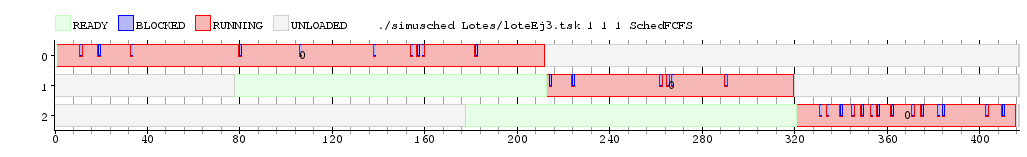
\includegraphics[width=1.1\textwidth]{imagenes/BatchExperimento.png}
  \caption{loteEj3.tsk con FCFS con un core}
\end{figure}

Podemos ver que se ejecutan pequeñas llamadas bloqueantes, estas tienen duración de un ciclo. 

\begin{figure}[H]
  \centering
    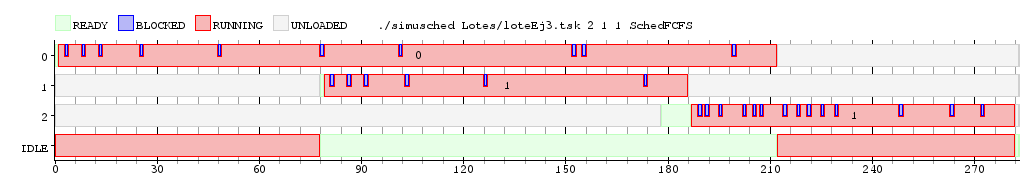
\includegraphics[width=1.1\textwidth]{imagenes/BatchExperimento2cores.png}
  \caption{loteEj3.tsk con FCFS con dos cores}
\end{figure}

Mismo experimento con dos cores en lugar de uno.